\chapter{Evolution of the Application Interface}


\textcolor{green}{aici e bine sa te referi la app (chiar daca e una simpla si cam doar GUI-ul e de ea); ar fi frumps sa ii spui sistem (chiar daca app e simpla, modelul de AI pe care-l integreaza e complex, deci nu e doar o app, e un adevarat sistem); mai mult ar fi dragutz sa ii gasesti un nume sugestiv la acest sistem si numele sa paara in tilul capitolului, cat si in titlul lucrarii de licenta}

\textcolor{ar fi bine ca acest capitol sa aiba urm structura:\\
1. fc-nalitati (e.g. load image and detect lessions)\\
2. design (info despre use-case(s), diagrama de arhitectura a app, diagrama de concepte/clase, diagr de secventa)\\
3. implementation (e.g. libraries used,technologies, languages, etc)\\
4. testing and validation (e.g. how you tested the app, some code assertions - it's ok for simple code, not for AI code)\\}

When coming up with designs for the interface and researching various Python libraries for GUIs, I came across the Gradio interface that is used specifically for machine learning models. Using this library, there are two ways to submit an image to the model for predictions: uploading the image from the device or submitting an already uploaded image from an array of them. This array represents images used as examples, which in my case reside in a directory in the project's root. \\
Implementing such an interface using the Gradio library was fairly simple, but I also wanted to display the correct label of the photo submitted along with the predictions. Because the way this library sends the data from the image selected doesn't include the actual name of the filename, I found myself thinking of ways to find and display the true label of the images selected from the examples. To do so, I compared the contents of each of the images existing in the directory to the contents of the image selected. In preparation for this, for each image saved as index.png, index being a variable from 1 to 151, I saved an additional file named index-label.txt, where label is either 0 or 1, corresponding to the labels normal or cancer. For the images uploaded from the user's device, there is no way to find the true label of the input, therefore, I added another class, unknown, that is displayed whenever the label of the image cannot be determined.\\
Because I modified the problem from a 4-label classification to a 2-label classification, I chose to train another label trained in detecting actionable-type images from the benign and malign ones. This second model is only used if the first model predicts the image as not being normal. I do this because the third model, which detects the bounding boxes, is trained on benign and malign images, and along with the coordinates of the boxes, it provides the classification of the input. The image below shows the interface of the application that detects inputs using the first model.\\
\begin{figure}[ht!]
    \centering
    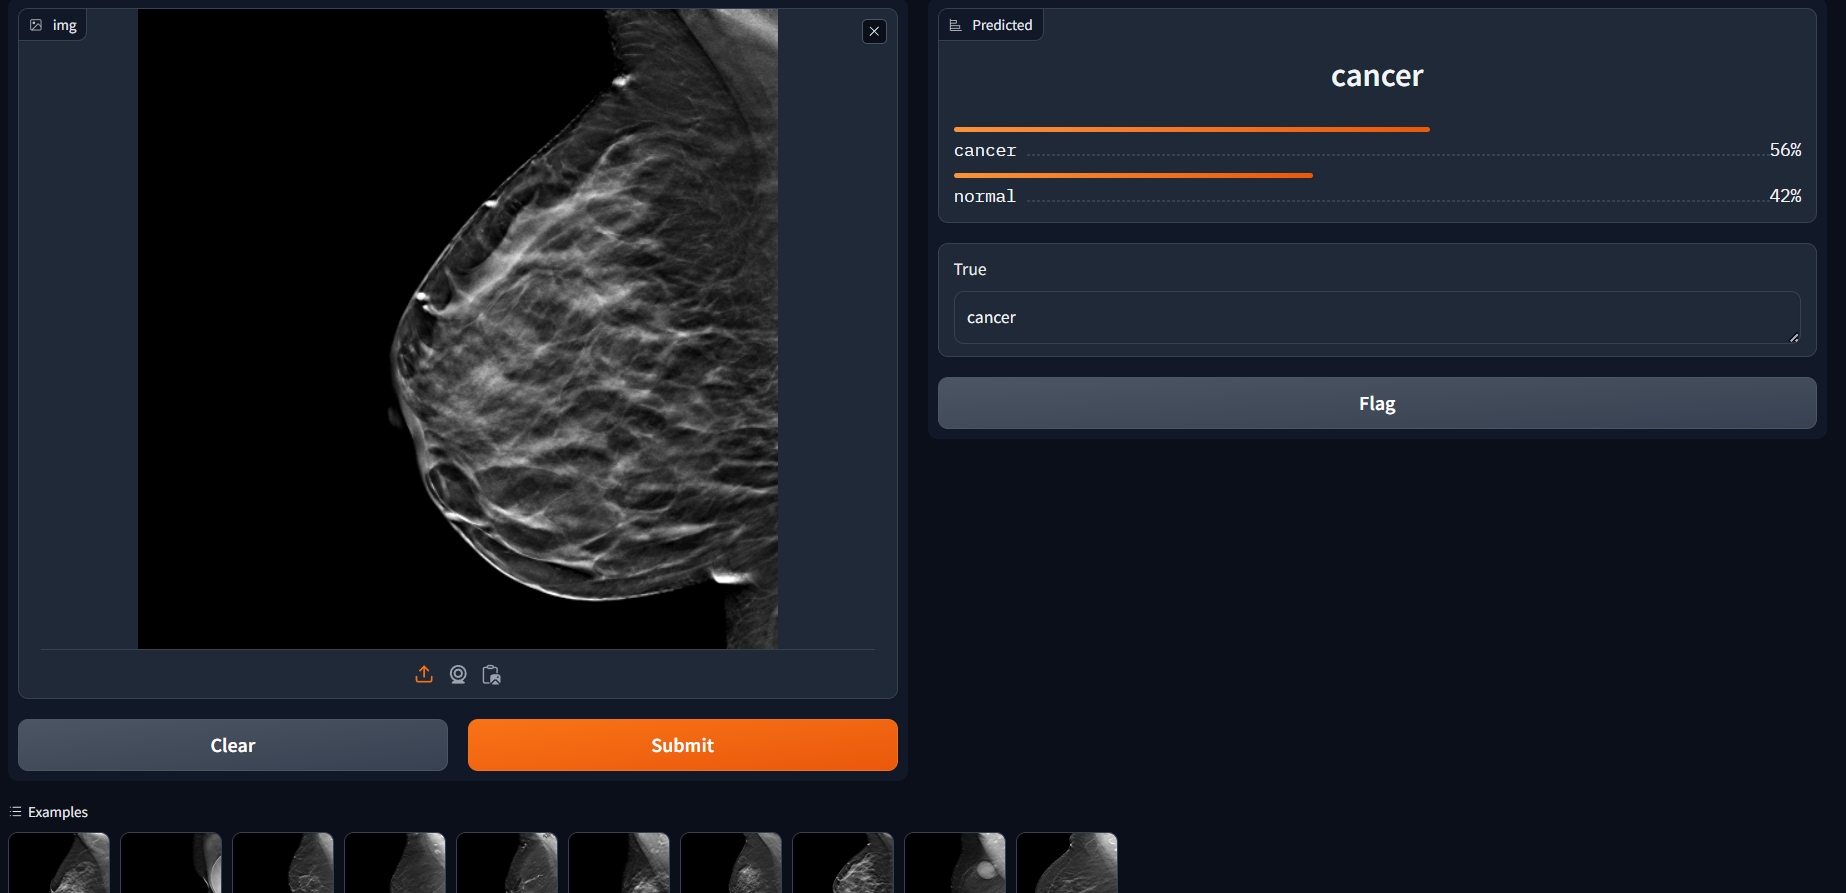
\includegraphics[width=0.75\linewidth]{figures/Figure16.png}
    \caption{Application interface}
    \label{fig:fig15}
\end{figure}